\documentclass[]{emse-exo}

\annee{CIS}
\module{MASTER MAVIM}
\matiere{Traitement d'Image Avanc�}
\type{TP}


\begin{document}

\sujet{Filtrage morphologique}

\note{Ce TP a pour objectif d'appr�hender le filtrage morphologique et notamment les filtres g�od�siques (par reconstruction).
}

\noindent Les diff�rents traitements seront r�alis�s sur l'image suivante :
\begin{figure}[h]
\begin{center}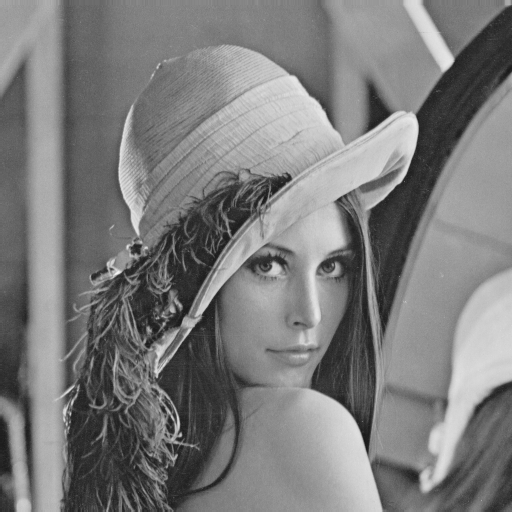
\includegraphics[width=3.25cm]{lena.png}
\end{center}
\end{figure}
\vspace*{-1cm}

\begin{exo}{Centre morphologique}
Le centre morphologique est un filtre auto-dual construit � partir d'une famille d'op�rateurs $\{\psi_i\}_i$ :
\begin{eqnarray}
C(f)=(f \vee (\wedge\{\psi_i(f)\})) \wedge (\vee\{\psi_i(f)\})
\end{eqnarray}

\begin{enumerate}
	\item Impl�menter cette transformation avec la famille $\{\gamma\phi\gamma, \phi\gamma\phi\}$ o� $\gamma$ d�signe l'ouverture morphologique et $\phi$ la fermeture morphologique.
	\item Tester cette transformation en faisant varier la taille de l'�l�ment structurant.
	\item Bruiter l'image 'Lena' avec un bruit 'poivre et sel' et comparer le centre morphologique avec le filtre m�dian.
\end{enumerate}
\end{exo}

\begin{exo}{Filtres altern�s s�quentiels (FAS)}
Les FAS peuvent �tre construits � partir d'une famille d'ouvertures et de fermetures morphologiques :
\begin{eqnarray}
N_i(f)&=&\gamma_i\phi_i\circ\gamma_{i-1}\phi_{i-1}\dots\gamma_2\phi_2\circ\gamma_1\phi_1(f)\\
M_i(f)&=&\phi_i\gamma_i\circ\phi_{i-1}\gamma_{i-1}\dots\phi_2\gamma_2\circ\phi_1\gamma_1(f)
\end{eqnarray}
o� $\gamma_k$ (resp. $\phi_k$) d�signe l'ouverture (resp. la, fermeture) morphologique avec un �l�ment structurant de taille $k$.
\begin{enumerate}
	\item Impl�menter ces deux transformations.
	\item Tester cette transformation sur l'image bruit�e en faisant varier la taille maximale $i$ de l'�l�ment structurant.
\end{enumerate}
\end{exo}

\begin{exo}{Filtres par reconstruction}
Rappelons tout d'abord l'op�ration de dilatation g�od�sique unitaire et de taille $n$ :
\begin{eqnarray}
\delta_f(g)&=&\wedge(\delta_{B_1}(g),f)\\
\delta_f^{n}(g)&=&\delta_f(\delta_f\dots(\delta_f(g)))
\end{eqnarray}
o� $\delta_{B_1}$ d�signe la dilatation morphologique avec un disque de rayon $1$ pour �l�ment structurant.
L'ouverture et la fermeture par reconstruction sont alors d�finis de la mani�re suivante :
\begin{eqnarray}
\gamma_k^{rec}(f)&=&\vee\{\delta_f^{n}(\epsilon_{B_k}(f)),n>0\}\\
\phi_k^{rec}(f)&=&M-\gamma_k^{rec}(M-f)
\end{eqnarray}
o� $\epsilon_{B_k}$ d�signe l'�rosion morphologique avec un disque $B$ de rayon $k$ pour �l�ment structurant.
\begin{enumerate}
	\item Impl�menter ces deux transformations.
	\item Tester cette transformation en faisant varier la taille $k$ de l'�l�ment structurant.
	\item Impl�menter et tester, sur l'image bruit�e, les filtres de centre morphologique et FAS avec ces op�rateurs g�od�siques et les comparer aux filtres usuels (notamment m�dian).
\end{enumerate}
\end{exo}

\end{document}